%%%%%%%%%%%%%% Figure 1: 8-K Merging Process
\begin{figure}
	\caption{8-K Matching Process} \label{fig1}
	\begin{center}
		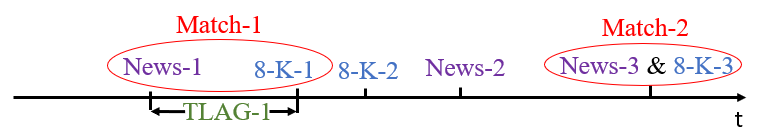
\includegraphics[scale=0.7]{../output/fig/fig1_matching.png}
	\end{center}
\end{figure}

Figure 1 illustrates the 8-K sample matching process. We match every 8-K day to its nearest news day. The news day can be earlier than (Match-1), the same as (Match-2) or later than (Match-3) the 8-K day. TLAG is defined as the number of days elapsed between the 8-K filing date and its nearest news day.

%%%%%%%%%%%%%%% Figure 2: 8-K Item Distribution
%\begin{figure}[htbp]
%	\begin{center}
%		\caption{8-K Item Distribution} \label{fig2}
%		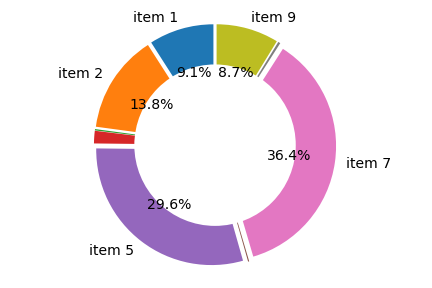
\includegraphics[scale=0.5]{../output/fig/fig2_8-K_before.png}
%		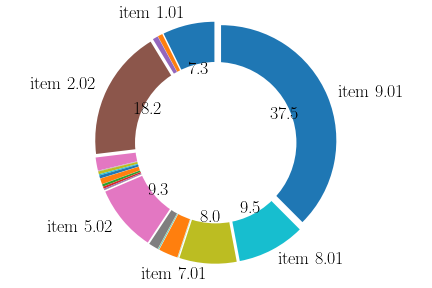
\includegraphics[scale=0.5]{../output/fig/fig2_8-K_after.png}
%	\end{center}
%\end{figure}
%
%Figure 2 illustrates the 8-K item distribution before (left) and after (right) August 23 of 2004. Each share of pie chart shows the percentage of corporate events reported under each 8-K items. See 8-K item list in \hyperref[appa]{Appendix A}.